%	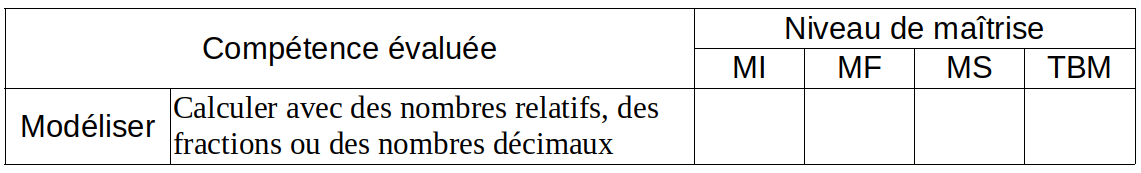
\includegraphics[scale=0.4]{competences}

\section{Calculer}
Calculer les expressions suivantes en détaillant tous les calculs:
\begin{questions}
	
	
	\question[3]  $A = 7 + 5 \times 8 - 2$
	
	\fillwithdottedlines{6cm}
	
	\question[3]  $B = 33 + 45 - 22 + 11$
	
	\fillwithdottedlines{6cm}
	
	\newpage
	
%	\question[4]  $C = 14 + 18 \div 3 + 25$
%	
%	\fillwithdottedlines{6cm}
	
	
	
	\question[4]  $D = 42 \div 7 + 34 - 3$
	
	\fillwithdottedlines{5.5cm}
	
	\question[4]  $E = (\num{18.1} + \num{4.6} + \num{2.3}) \div 5 + \num{2.5}$
	
	\fillwithdottedlines{5.5cm}
	
\end{questions}

	\section{Traduire}
Traduire les expressions suivantes par une phrase, sans faire les calculs.
\begin{questions}
	
	\question[3]  $E = 45 \times 4 + 5$
	\fillwithdottedlines{3cm}
	
	
	\question[3]  $F = (23 \div 5) - (7 \times 3)$
	\fillwithdottedlines{3cm}
	
\end{questions}


